\documentclass[a4paper]{article}


\usepackage[english]{babel}
\usepackage[a4paper,top=3cm,bottom=2cm,left=3cm,right=3cm,marginparwidth=1.75cm]{geometry}
\usepackage{amsmath}
\usepackage{bm} %bold for math formulas
\usepackage{amsfonts} %mathematical fields fonts
\usepackage{float} %images held
\usepackage[colorinlistoftodos]{todonotes}
\usepackage[colorlinks=true, allcolors=blue]{hyperref}
\usepackage[table]{colortbl}
\usepackage{multirow}
\usepackage{siunitx}

\title{Integrated Systems Architecture\\Lab2 Report}
\author{Marco Andorno 247222\\Michele Caon\\Matteo Perotti 251453\\Giuseppe Sarda}

\begin{document}
\maketitle

\section{Comparison between different combinations of adders and multipliers}
Starting from the pipelined and retimed architecture developed in Lab 1, we exploited Synopsys DesignWare Library to compare several design metrics using different implementations for the arithmetic operators used in our design.

Among others, DesignWare makes available the following synthesis models of adders and multipliers:
\begin{itemize}
	\item \texttt{DW01\_add} \footnote{As the feedback branch of the filter gets subtracted from the input in direct form II, Synopsys actually uses also a subtractor (\texttt{DW01\_sub}), for which the same implementations as the adder are available. So when we say that we used a certain kind of adder, we mean that we used it for all adders and for that subtractor too.}:
	\begin{itemize}
		\item \texttt{rpl}: ripple-carry adder
		\item \texttt{cla}: carry-look-ahead adder
		\item \texttt{pparch}: delay optimized flexible parallel-prefix adder
	\end{itemize}
	\item \texttt{DW02\_mult}:
	\begin{itemize}
		\item \texttt{csa}: carry-save array multiplier
		\item \texttt{pparch}: delay optimized flexible Booth-recoded Wallace tree multiplier
	\end{itemize}
\end{itemize}

The approach used is totally similar to the one suggested for the first laboratory experience:
\begin{itemize}
	\item Synthesize design using Design Compiler, setting the clock period do 0 in order to find the maximum frequency $f_{max}$.
	\item Synthesize again using a clock period corresponding to $f_{max}/4$ and find out the area of the design.
	\item Simulate on a sufficient number of samples (1000 was the sweet spot to trade off accuracy and simulation time) in ModelSim to extract the switching activity.
	\item Run Design Compiler once again to carry out the power estimation.
\end{itemize}

\subsection{Maximum frequency}
Table \ref{tab:fmax} show the maximum frequency achieved for each pair of implementations. Red and green cells highlight respectively the lowest and highest maximum frequencies. Note that the best frequency achieved is the same that Synopsys reached by choosing the implementations on its own in the previous laboratory experience (in fact, the resources report of that base version shows exactly that \texttt{pparch} was chosen as the architecture of both the adders and the multipliers).
% Please add the following required packages to your document preamble:
% \usepackage{multirow}
% \usepackage[table,xcdraw]{xcolor}
% If you use beamer only pass "xcolor=table" option, i.e. \documentclass[xcolor=table]{beamer}
\begin{table}[hbtp]
	\centering
	\begin{tabular}{clllll}
	\cline{1-5}
	\multicolumn{2}{|c|}{}                                                           & \multicolumn{3}{c|}{Adder}                                                                                                           &  \\ \cline{3-5}
	\multicolumn{2}{|c|}{\multirow{-2}{*}{$f_{max}$ [\si{\mega\hertz}]}}               & \multicolumn{1}{l|}{rpl}                           & \multicolumn{1}{l|}{cla}   & \multicolumn{1}{l|}{pparch}                        &  \\ \cline{1-5}
	\multicolumn{1}{|c|}{}                             & \multicolumn{1}{l|}{csa}    & \multicolumn{1}{l|}{\cellcolor[HTML]{FFCCC9}285.7} & \multicolumn{1}{l|}{287.4} & \multicolumn{1}{l|}{285.7} &  \\ \cline{2-5}
	\multicolumn{1}{|c|}{\multirow{-2}{*}{Multiplier}} & \multicolumn{1}{l|}{pparch} & \multicolumn{1}{l|}{431.0}                         & \multicolumn{1}{l|}{684.9} & \multicolumn{1}{l|}{\cellcolor[HTML]{9AFF99}689.7} &  \\ \cline{1-5}
	\multicolumn{1}{l}{}                               &                             &                                                    &                            &                                                    & 
	\end{tabular}
	\caption{Maximum frequency}
	\label{tab:fmax}
\end{table}

\begin{figure}[hbtp]
	\centering
	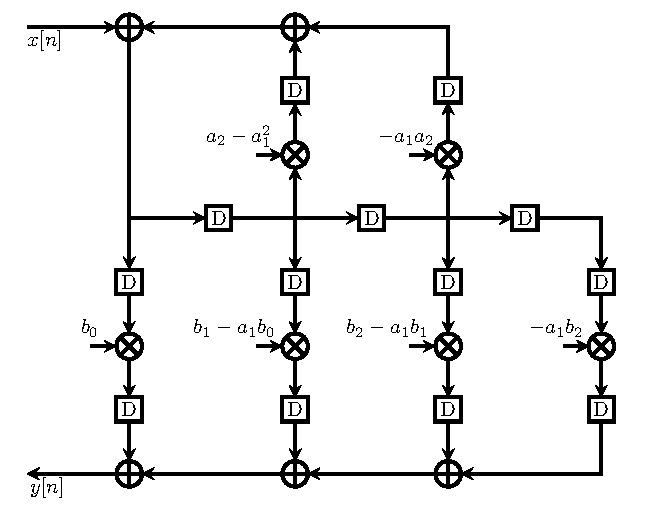
\includegraphics[width=.6\linewidth]{media/pipelined_lookahead_dfg.pdf}
	\caption{DFG of the filter}
	\label{fig:dfg}
\end{figure}
Figure \ref{fig:dfg} shows the DFG of the final architecture achieved at the end of the previous lab, by looking at which, one can quite positively state that the critical path is the delay of a single multiplier $T_m$, as it is almost certainly larger than the delay of three adders $3T_a$.
So one would expect the maximum frequency to remain constant as long as the multiplier used is the same and only the implementation of the adder is changed.

In fact, this is what happens in five cases out of six in table \ref{tab:fmax}: when using the carry-save based multiplier, the clock frequency is always limited by its delay, irrespective of the adder used. But when using the faster multiplier (\texttt{pparch}), the slowest ripple-carry adder seems to be the limiting factor, as the maximum frequency it allows is much lower than the one achieved with the same multiplier but faster adders.

So in this case the critical path seems to be the series of three adders, instead of the single multiplier. To verify this hypothesis, the DFG of the filter was slightly modified by introducing an additional pipeline stage to split the chain of $3$ adders into $2+1$ adders, as there is a feedforward cutset that allows it. By repeating the synthesis flow using the ripple-carry adder and the parallel prefix multiplier, the maximum frequency increased by around 10\%, from \SI{431.0}{\mega\hertz} to \SI{473.9}{\mega\hertz}. Even if this is not a 33\% improvement (probably due to design optimizations operated by the tool), as conceptually expected, it can nevertheless be concluded that the chain of three 24-bit ripple-carry adders was in the end the bottleneck of the design, being slower than one single 24-bit parallel prefix multiplier.

All in all, choosing the parallel-prefix multiplier combined with either carry-loohahead or parallel-prefix adders is the best option for speed: the maximum clock frequency is 60\% higher than the pair \texttt{pparch} multiplier/\texttt{rpl} adder, and 242\% faster than all carry-save multiplier based implementations.

\subsection{Cell area}
For what concerns area, table \ref{tab:area} shows that this figure seems to be once again mostly a matter of the type of multiplier chosen. Choosing the parallel-prefix multiplier is again the winning choice, as such implementations have a total area 38\% smaller than the one of designs based on a carry-save multiplier. 

In the case of area, the choice of the type of adder does not seem to influence much the final figure, showing variations of less than 1\% among the three implementation, given the multiplier type.
\begin{table}[hbtp]
	\centering
	\begin{tabular}{clllll}
	\cline{1-5}
	\multicolumn{2}{|c|}{}                                                           & \multicolumn{3}{c|}{Adder}                                                                                                                                         &  \\ \cline{3-5}
	\multicolumn{2}{|c|}{\multirow{-2}{*}{Area [\si{\micro\meter^2}]}}                         & \multicolumn{1}{l|}{rpl}                             & \multicolumn{1}{l|}{cla}                             & \multicolumn{1}{l|}{pparch}                          &  \\ \cline{1-5}
	\multicolumn{1}{|c|}{}                             & \multicolumn{1}{l|}{csa}    & \multicolumn{1}{l|}{20987.4} & \multicolumn{1}{l|}{\cellcolor[HTML]{FFCCC9}21113.5} & \multicolumn{1}{l|}{20978.1} &  \\ \cline{2-5}
	\multicolumn{1}{|c|}{\multirow{-2}{*}{Multiplier}} & \multicolumn{1}{l|}{pparch} & \multicolumn{1}{l|}{15282.8} & \multicolumn{1}{l|}{15408.8} & \multicolumn{1}{l|}{\cellcolor[HTML]{9AFF99}15273.5} &  \\ \cline{1-5}
	\multicolumn{1}{l}{}                               &                             &                                                      &                                                      &                                                      & 
	\end{tabular}
	\caption{Total area}
	\label{tab:area}
\end{table}

\subsection{Total power dissipation}
Power dissipation is clearly where the advantage of the parallel-prefix multiplier falls short. All implementations based on that show a 32-fold increase in dynamic power and a 14-fold increase in leakage power.

As always in digital design, as well as in life, one cannot get the best of both worlds, but has to settle for a trade-off, in this case between speed and power, as usual.
\begin{table}[hbtp]
	\centering
	\begin{tabular}{clllll}
	\cline{1-5}
	\multicolumn{2}{|c|}{\multirow{2}{*}{Power [\si{\micro\watt}]}} & \multicolumn{3}{c|}{Adder}                                                                                                                                                                                                     &  \\ \cline{3-5}
	\multicolumn{2}{|l|}{}                                                                                                        & \multicolumn{1}{l|}{rpl}                                                 & \multicolumn{1}{l|}{cla}                                                 & \multicolumn{1}{l|}{pparch}                                              &  \\ \cline{1-5}
	\multicolumn{1}{|c|}{\multirow{2}{*}{Multiplier}}                        & \multicolumn{1}{l|}{csa}                           & \multicolumn{1}{l|}{\begin{tabular}[c]{@{}l@{}}120.1\\ 3.1\end{tabular}} & \multicolumn{1}{l|}{\begin{tabular}[c]{@{}l@{}}120.1\\ 3.1\end{tabular}} & \multicolumn{1}{l|}{\begin{tabular}[c]{@{}l@{}}120.1\\ 3.1\end{tabular}} &  \\ \cline{2-5}
	\multicolumn{1}{|c|}{}                                                   & \multicolumn{1}{l|}{pparch}                        & \multicolumn{1}{l|}{\begin{tabular}[c]{@{}l@{}}3815\\ 43.5\end{tabular}} & \multicolumn{1}{l|}{\begin{tabular}[c]{@{}l@{}}3816\\ 43.5\end{tabular}} & \multicolumn{1}{l|}{\begin{tabular}[c]{@{}l@{}}3816\\ 43.5\end{tabular}} &  \\ \cline{1-5}
																			 &                                                    &                                                                          &                                                                          &                                                                          & 
	\end{tabular}
	\caption{Dynamic and leakage power}
	\label{tab:pwr}
\end{table}

\subsection{Summing up}
If the main requirement is pure speed, then an architecture based on parallel-prefix Booth-recoded Wallace tree multipliers and carry-lookahed or parallel-prefix adders is the way to go.

If, on the other hand, the power budget is a limiting factor, one has to settle for lower processing speed and use CSA-based multipliers along with whichever adder they like best.

\section{MBE based Multiplier with Roorda's approach and Dadda Tree}
	Let's suppose to have a multiplication to be done between two numbers \textbf{x} and \textbf{y}.
	\begin{itemize}
		\item \textbf{x} is the multiplicand
		\item \textbf{y} is the multiplier
		\item $\bm{k_x}$ is the parallelism of \textbf{x}
		\item $\bm{k_x^{I}}$ is the number of bits representing the \textbf{I}nteger part of \textbf{x}
		\item $\bm{k_x^{F}}$ is the number of bits representing the \textbf{F}ractional part of \textbf{x}
		\item $\bm{k_y}$ is the parallelism of \textbf{y}
		\item $\bm{k_y^{I}}$ is the number of bits representing the \textbf{I}nteger part of \textbf{y}
		\item $\bm{k_y^{F}}$ is the number of bits representing the \textbf{F}ractional part of \textbf{y}
	\end{itemize}
	We want to perform the multiplication with the \textbf{MBE-radix4} encoded version of the multiplier \textbf{y}.
	This shrewdness allow us to reduce the number of partial products by half:
	indeed \textbf{y} is encoded with $\bm{k_y^{'}}$ symbols in $\{\pm{2}, \pm{1}, 0\}$.
	\begin{equation}
		\bm{k_y^{'} = \lceil \frac{k_y}{log_2(r)} \rceil = \lceil \frac{k_y}{2} \rceil}
	\end{equation}
	It's possible to MBE-encode a number in radix4 simply taking $\lceil \frac{k_y}{2} \rceil$ 1-bit overlapping triplets of it. 
	If we consider \textbf{y} represented as a sequence of bits $\bm{y_{(k_y-1)} y_{(k_y-2)} \ldots 
	y_{1} y_{0}}$ with the \textbf{LSB} in position \textbf{0}, then for correctly encoding \textbf{y} we must add
	a $\bm{y_{-1}}$ bit fixed at \textbf{0} to complete the first triplet. If $\bm{k_y}$ is odd then it will be
	added a bit $\bm{y_{k_y}}$ to complete also the last one.\\
	The encoded multiplier is then represented by the string of symbols
	\begin{equation}
		Y_{(\lceil \frac{k_y}{2} \rceil - 1)} Y_{(\lceil \frac{k_y}{2} \rceil - 2)} \ldots Y_{1} Y_{0}
	\end{equation}
	chosen from the set $\{\pm{2}, \pm{1}, 0\}$ wrt the following table
	\begin{table}[]
		\begin{tabular}{|c|c|}
			\hline
			$y_{n+1} y_n y_{n-1}$ & $Y_{n}$  \\ \hline
			000 & 0  \\ \hline
			001 & 1  \\ \hline
			010 & 1  \\ \hline
			011 & 2  \\ \hline
			100 & -2 \\ \hline
			101 & -1 \\ \hline
			110 & -1 \\ \hline
			111 & 0  \\ \hline
		\end{tabular}
	\end{table}
	The product is now between \textbf{x} and \textbf{Y} the MBE-radix4 encoded version of \textbf{y}.
	Each partial product between a symbol of \textbf{Y} and \textbf{x} is performed using a multiplexer: two of 
	the three bits which encode a symbol are used as control lines for the mux which can let pass either \textbf{0}, 
	or \textbf{x}, or \textbf{2x}. The other encoding bit is asserted only if the symbol is negative and it is used
	to complement the partial product. Moreover it will be added to the LSB of its partial product, to ensure a
	correct 2's complement negation. This way it's easy to obtain all the possible partial product: \textbf{0}, 
	\textbf{x}, \textbf{-x}, \textbf{-2x} and \textbf{2x}.

	Since the entire operation has to last one clock cycle all the partial products are obtained in parallel by the same number of encoding circuits and multiplexers. The derived tree is thought as a Dadda Tree and the number of FA is reduced
	simplifying the extended sign bits as proposed in \cite{roorda:1}.
	We have $\lceil \frac{k_y}{2} \rceil $ partial products to be compressed to only two terms with a Dadda Tree of CSA. The 
	situation is the following:
% table with the current situation
	Since we are not working with full precision, we can do not consider the first $\bm{k_y^I}$ MSBs, because they do not
	impact on the others. The $\bm{k_y^F}$ LSBs are on the contrary fundamental because of the carry of the sums in which they are involved.
	As Roorda highlighted, the bits of sign-extension can be thought as a series of \textbf{1} if the complement of the sign bit is added in its original position.
	This leads to a further optimization, because each column of \textbf{1}, starting from the rightmost one, can be simplified
	in advance knowing that
	\begin{equation}
		\begin{cases}
        	?\ \ 1\\
        	?\ \ 1\\
        \end{cases}
        \implies
        \begin{cases}
        	?\ \ 0\\
        	?\ \ 0\\
        	1\ \ 0\\
        \end{cases}
	\end{equation}
	and
	\begin{equation}
		\begin{cases}
        	?\ \ 1\\
        	?\ \ a\\
        \end{cases}
        \implies
        \begin{cases}
        	?\ \ \bar{a}\\
        	?\ \ 0\\
        	a\ \ 0\\
        \end{cases}
	\end{equation}
	At the end we have the first row in which there is a string of "\textbf{10}", followed by a sequence of "$\bm{1\ \bar{p}_{k_{x}+1}^i}$" and then a triplet composed of "$\bm{\bar{p}_{k_{x}+1}^0 p_{k_{x}+1}^0 p_{k_{x}+1}^0}$". On the second row, under the first element $\bm{\bar{p}_{k_{x}+1}^0}$ of this triplet, there is $\bm{\bar{p}_{k_{x}+1}^1}$.\\
	\paragraph{Design of the multiplier} In our design we have
		\begin{itemize}
			\item $\bm{k_x = k_y = 24}$
			\item $\bm{k_x^{I} = k_y^{I} = 2}$
			\item $\bm{k_x^{F} = k_y^{I} = 22}$
			\item \textbf{12} partial products
			\item at most $\bm{\frac{k_y}{2}+1 = 13}$ elements in a single column
		\end{itemize}
		In a single column we can count up to 13 elements, because the MUX let pass only \textbf{x} multiplied for the absolute value of the symbol \textbf{Y}. The "negative" bit (one of the three which encode a single symbol) it has to be added 
		to the LSB of its partial product: therefore we have 12+1 elements at most in a column.
		This is not so bad, because with the Dadda Tree we are still in the case of having only 5 levels of FA (13 elements in 
		a column at most). 
	\bibliography{ISA-lab2_report}
	\bibliographystyle{ieeetr}
\end{document}